\documentclass{article}
\usepackage[polish]{babel}
\usepackage[T1]{fontenc}
\usepackage{amsmath}
\usepackage{float}
\usepackage{graphicx} % Required for inserting images
\graphicspath{ {./images/} }

\title{Laboratorium 9 \\ Równania różniczkowe zwyczajne - część I}
\author{Maciej Borowiec}
\date{21.05.2025}

\begin{document}

\maketitle

\section{Wprowadzenie}
Celem ćwiczenia było zrobienie sześciu zadań związanych z równaniami różniczkowymi zwyczajnymi. Zadania miały na celu przedstawienie sposobów rozwiązywania równań różniczkowych.

\section{Zadania}

\subsection{Zadanie 1.}
Zadanie polegało na przekształceniu podanych równań różniczkowych na równoważny układ równań pierwszego rzędu.

\subsubsection{Równanie Van der Pol'a}
$$y'' = y'(1- y^2) - y$$
Podstawiamy $u_1 = y$, $u_2 = y'$, wtedy:
\begin{equation}
    \begin{cases}
        u_1' = u_2 \\
        u_2' = u_2(1-u_1^2)-u_1
    \end{cases} \nonumber
\end{equation}
Otrzymany układ równań jest układem równań pierwszego rzędu.

\subsubsection{Równanie Blasiusa}
$$y''' = -yy''$$
Podstawiamy $u_1 = y$, $u_2 = y'$, $u_3 = y''$, wtedy:
\begin{equation}
    \begin{cases}
        u_1' = u_2 \\
        u_2' = u_3 \\
        u_3' = -u_1u_3
    \end{cases} \nonumber
\end{equation}
Ponownie otrzymano układ równań pierwszego rzędu.

\subsubsection{II zasada dynamiki Newtona dla problemu dwóch ciał}
\begin{equation}
    \begin{cases}
        y_1'' = -GMy_1/(y_1^2+y_2^2)^{3/2} \\
        y_2'' = -GMy_2/(y_1^2+y_2^2)^{3/2}
    \end{cases} \nonumber
\end{equation}
Podstawiamy $u_1 = y_1$, $u_2 = y_2$, $u_3 = y_1'$, $u_4 = y_2'$, wtedy:
\begin{equation}
    \begin{cases}
        u_1' = u_3 \\
        u_2' = u_4 \\
        u_3' = -GMu_1/(u_1^2+u_2^2)^{3/2} \\
        u_4' = -GMu_2/(u_1^2+u_2^2)^{3/2}
    \end{cases} \nonumber
\end{equation}
Otrzymany układ równań jest układem równań pierwszego rzędu.

\subsection{Zadanie 2.}
W tym zadaniu należało przekształcić poniższy problem początkowy do autonomicznego problemu początkowego.
\begin{equation}
    \begin{cases}
        y_1' = \frac{y_1}{t} + y_2t \\
        y_2' = \frac{t}{y_1}(y_2^2 - 1) \\
    \end{cases} \nonumber
    \begin{cases}
        y_1(1) = 1 \\
        y_2(1) = 0 \\
    \end{cases} \nonumber
\end{equation}
\\
Aby poprawnie przekształcić problem do problemu początkowego, należy dodać nową zmienną tożsamościowo równą $t$. W tym przypadku dodajemy zmienną $y_3(t) = t$. Wtedy otrzymujemy:
\begin{equation}
    \begin{cases}
        y_1' = \frac{y_1}{y_3} + y_2y_3 \\
        y_2' = \frac{y_3}{y_1}(y_2^2 - 1) \\
        y_3' = 1
    \end{cases} \nonumber
    \begin{cases}
        y_1(1) = 1 \\
        y_2(1) = 0 \\
        y_3(1) = 1
    \end{cases} \nonumber
\end{equation}
W ten sposób otrzymaliśmy autonomiczny problem początkowy.

\subsection{Zadanie 3.}
Dla danego problemu początkowego:
\begin{equation}
    y' = \sqrt{1-y}
\end{equation}
$$y(0) = 0$$
Należało pokazać, że funkcja $y(t) = \frac{t}{4}(4-t)$ spełnia równanie i warunek początkowy oraz wyznaczyć dziedzinę, dla której ta funkcja jest rozwiązaniem tego problemu.
\\\\
Sprawdzenie warunku początkowego:
$$y(0) = \frac{0}{4}(4-0) = 0$$
Następnie wyznaczmy pochodną funkcji $y(t)$:
$$y'(t) = (\frac{t}{4}(4-t))' = (t - \frac{t^2}{4})' = 1 - \frac{t}{2}$$
Podstawmy do problemu początkowego (1):
$$1-\frac{t}{2} = \sqrt{1 - t + \frac{t^2}{4}} = \sqrt{(1-\frac{t}{2})^2}$$
$$1-\frac{t}{2} = |1-\frac{t}{2}|$$
Zatem dana funkcja jest rozwiązaniem tego problemu wtw., gdy $1-\frac{t}{2} \geq 0$.
$$1-\frac{t}{2} \geq 0 $$
$$t \leq 2$$
Zatem dziedziną tego rozwiązania jest $D = (-\infty;2]$.

\subsection{Zadanie 4.}
W tym zadaniu należało przeanalizować dane równanie różniczkowe zwyczajne i porównać metody Eulera (jawną oraz niejawną) dla tego równania.
\\\\
Dane jest równanie:
\begin{equation}
    y' = -5y
\end{equation}
z warunkiem początkowym $y(0) = 1$. Równanie rozwiązujemy numerycznie dla kroku $h = 0.5$.

\subsubsection{Analityczna stabilność}
Należy sprawdzić, czy rozwiązania tego równania są stabilne.
\\\\
Weźmy:
\begin{equation}
    \begin{cases}
        y' = -5y \\
        y(0) = 1
    \end{cases} \nonumber
    \begin{cases}
        z' = -5z \\
        z(0) = z_0
    \end{cases} \nonumber
\end{equation}
Wtedy rozwiązania równania (2) są stabilne, gdy:
\begin{equation}
    \forall\varepsilon>0\ \ \exists\delta: ||z(t_0) - y(t_0)|| < \delta \implies ||z(t) - y(t)|| < \varepsilon \text{ dla } t \geq t_0
\end{equation}
Jako, że dane równania są równaniami testowymi Dahlquist'a to znamy ich rozwiązania: $y(t) = e^{-5t}$, $z(t) = z_0e^{-5t}$. Wiemy również, że $t_0 = 0$, $y(t_0) = 1$, $z(t_0) = z_0$. Po przekształceniu warunku (3) otrzymujemy:
$$\forall\varepsilon>0\ \ \exists\delta: |z_0 - 1| < \delta \implies |z_0e^{-5t} - e^{-5t}| < \varepsilon \text{ dla } t \geq 0$$
Dowód przeprowadźmy zaczynając od poprzednika implikacji:
$$|z_0 - 1| < \delta$$
Przemnóżmy obie równania przez $e^{-5t}$ ($>0$):
$$|z_0e^{-5t} - e^{-5t}| < \delta e^{-5t}$$
Dla dowolnego $\varepsilon>0$ możemy wziąć $\delta = \varepsilon$:
$$|z_0e^{-5t} - e^{-5t}| < \varepsilon e^{-5t}$$
Dla $t \geq 0$ zachodzi $e^{-5t} \geq 1$, zatem:
$$|z_0e^{-5t} - e^{-5t}| < \varepsilon e^{-5t} \leq \varepsilon \text{ dla } t \geq 0$$
Ostatecznie:
$$|z_0e^{-5t} - e^{-5t}| < \varepsilon \text{ dla } t \geq 0$$
Otrzymaliśmy następnik implikacji w warunku, zatem rozwiązania równania (2) są stabilne. Są one również stabilne asymptotycznie, gdyż:
$$\lim_{t\to\infty} |z_0e^{-5t} - e^{-5t}| = 0$$

\subsubsection{Zbieżność metody Eulera}
Należy udowodnić zbieżność metody Eulera, tzn., że:
\begin{equation}
    \lim_{\substack{h\to0 \\ n\to+\infty \\ nh = t}}y_n = y(t)
\end{equation}
gdzie $y(t)$ to wartość rozwiązania analitycznego w punkcie $t=nh$, a $y_n$ to wartość rozwiązania numerycznego w tym punkcie.
\\\\
Wiemy, że:
$$y_n = y_{n-1} + h(-5y_{n-1}) = y_{n-1}(1-5h) = y_{n-2}(1-5h)(1-5h) =\ ...$$
Zatem:
$$y_n = y_0(1-5h)^n = (1-5h)^n$$
Używając $nh = t \implies n = \frac{t}{h}$:
$$y_n = (1 - 5h)^{\frac{t}{h}} = (1 + (-5h))^{\frac{1}{-5h}\cdot(-5t)}$$
Używając własności $\lim_{s\to0} (1+s)^{\frac{1}{s}} = e$, po podstawieniu do lewej strony równania (4):
$$L = \lim_{\substack{h\to0 \\ n\to+\infty \\ nh = t}}(1 + (-5h))^{\frac{1}{-5h}\cdot(-5t)} = e^{-5t} = y(t) = P$$
Lewa strona równania równa się prawej, zatem metoda Eulera jest zbieżna.

\subsubsection{Numeryczna stabilność metod Eulera}
Należało sprawdzić czy metoda Eulera jawna oraz niejawna są stabilne dla tego równania z zadanym krokiem $h=0.5$.
\\\\
Metoda Eulera jawna jest stabilna, gdy:
$$|1+h\lambda| < 1$$
Podstawiając $h=0.5$ i $\lambda = -5$ ($y'=-5y=\lambda y$):
$$|1+0.5*(-5)| = |1-2.5| = 1.5 < 1$$
Zachodzi sprzeczność, zatem metoda Eulera jawna nie jest stabilna w tym przypadku.
\\\\
Metoda Eulera niejawna jest stabilna, gdy:
$$\bigg|\frac{1}{1-h\lambda}\bigg| < 1$$
Podstawiając $h=0.5$ i $\lambda = -5$:
$$\bigg|\frac{1}{1-(-2.5)}\bigg| = \bigg|\frac{1}{3.5}\bigg| = \frac{2}{7} < 1$$
Ta nierówność jest spełniona, więc metoda Eulera niejawna jest stabilna dla danego równania i kroku $h$.

\subsubsection{Numeryczne rozwiązanie dla $t=0.5$}
Należało policzyć wartość rozwiązania dla $t=0.5$ używając obu metod Eulera. Otrzymane wyniki przedstawione są w tabeli poniżej.
\begin{table}[h!]
    \centering
    \begin{tabular}{|c|c|c|}
        \hline
        Typ rozwiązania & Otrzymana wartość & Błąd \\
        \hline
        Analityczne & $0.082085$ & $0$ \\
        Euler - jawne & $-1.5$ & $1.582084$ \\
        Euler - niejawne & $0.285714$ & $0.203629$ \\
        \hline
    \end{tabular}
    \caption{Wartości rozwiązań w punkcie $0.5$ dla kroku $0.5$}
    \label{table}
\end{table}
\\
Z danej tabeli (Tabela 1) widać, że metoda niejawna otrzymała bardziej dokładny wynik, lecz obie metody są mało dokładne. Jest tak, ponieważ wykonują one tylko jeden, duży krok.

\subsubsection{Poprawienie rozwiązania dla $t=0.5$}
Chcemy poprawić rozwiązanie, by błąd w tym punkcie nie przekraczał $0.001$. W tym celu będziemy zmniejszać krok $h$ do momentu osiągnięcia podanej tolerancji. Otrzymane rozwiązania zostały przedstawione w tabeli poniżej.
\begin{table}[h!]
    \centering
    \begin{tabular}{|c|c|c|c|c|}
        \hline
        Typ rozwiązania & Krok $h$ & Liczba kroków & Wartość w $0.5$ & Błąd \\
        \hline
        Euler - jawne & $0.001938$ & $258$ & $0.08109$ & $0.000995$ \\
        Euler - niejawne & $0.009434$ & $53$ & $0.08300$ & $0.000915$ \\
        \hline
    \end{tabular}
    \caption{Poprawione wartości rozwiązań w punkcie $0.5$}
    \label{table}
\end{table}
\\
Jak widać w tabeli (Tabela 2), metoda niejawna Eulera okazała się dużo lepsza w tym przypadku. Otrzymuje ona dokładny wynik prawie 5 razy szybciej niż metoda jawna. Dzięki temu maksymalny krok $h$, który otrzymuje poprawny wynik dla danej tolerancji, jest 5 razy większy dla metody niejawnej w porównaniu z metodą jawną.

\subsubsection{Bezpośrednia iteracja w niejawnej metodzie Eulera}
Do wyznaczenia wartości $y_{n+1}$ w niejawnej metodzie Eulera użyto metody bezpośredniej iteracji:
$$y_{n+1}^{(0)} = y_n$$
$$y_{n+1}^{(k+1)} =\phi(y_{n+1}^{(k)})$$
Pytamy o maksymalną dopuszczalną wartość kroku $h$, przy której metoda pozostanie zbieżna.
\\\\
Metoda niejawna Eulera w naszym przypadku wygląda następująco:
$$y_{n+1} = y_n + h(-5y_{n+1})$$
Zatem używając bezpośredniej iteracji:
$$y_{n+1}^{(k+1)} = y_n - 5hy_{n+1}^{(k)} = \phi(y_{n+1}^{(k)})$$
Do wyznaczenia kiedy metoda jest zbieżna użyjemy pochodnej.
$$\phi'(y_{n+1}^{(k)}) = -5h$$
Wartość bezwzględna pochodnej musi być mniejsza od 1.
$$|\phi'(y_{n+1}^{(k)})| < 1$$
$$|-5h| < 1$$
Krok musi być dodatni:
$$h < \frac{1}{5}$$
Zatem metoda jest zbieżna dla kroku $h < 0.2$.
\\\\
Naradza się pytanie, czy uzasadnione byłoby użycie metody Newtona do wyznaczenia $y_{n+1}$. Spójrzmy ponownie na wzór na $y_{n+1}$:
$$y_{n+1} = y_n + h(-5y_{n+1})$$
Jest to bardzo proste równanie liniowe, z którego można bez problemu wyznaczyć wzór jawny na $y_{n+1}$:
$$y_{n+1} + 5hy_{n+1} = y_n$$
$$y_{n+1}(1 + 5h) = y_n$$
$$y_{n+1}= \frac{y_n}{1 + 5h}$$
Jak widać, dla tak prostego przypadku, nie ma uzasadnienia do użycia metody Newtona, która się specjalizuje w rozwiązywaniu równań nieliniowych.

\subsection{Zadanie 5.}
Dla danego układu równań różniczkowych zwyczajnych:
\begin{equation}
    \begin{cases}
        y_1' = -2y_1 + y_2 \\
        y_2' = -y_1 - 2y_2
    \end{cases} \nonumber
\end{equation}
Należało wyznaczyć przedział wartości kroku $h$, dla którego metoda Eulera jest stabilna dla tego układu równań.
\\\\
Układ równań można przedstawić w postaci macierzowej:
$$y' = Ay$$
gdzie:
\begin{equation}
    y' =
    \begin{bmatrix}
        y_1' \\ y_2'
    \end{bmatrix}
    ,\quad
    A =
    \begin{bmatrix}
        -2 & 1 \\
        -1 & -2
    \end{bmatrix}
    ,\quad
    y =
    \begin{bmatrix}
        y_1 \\ y_2
    \end{bmatrix}
\nonumber
\end{equation}
Wtedy wiadomo, że metoda Eulera jest stabilna, gdy dla każdej wartości własnej $\lambda$ macierzy $A$ zachodzi:
$$|1 + \lambda h| < 1 $$
Wartości własne macierzy możemy wyznaczyć następująco:
$$\det(A-\lambda I) = 0 $$
\begin{equation}
    \begin{vmatrix}
        -2-\lambda & 1 \\
        -1 & -2-\lambda
    \end{vmatrix}
    = 0
\nonumber
\end{equation}
Wtedy:
$$(-2-\lambda)^2 + 1 = \lambda^2 + 4\lambda + 5 = 0$$
$$\Delta = 4^2 - 4*5 = -4, \quad \sqrt{\Delta} = \pm2i$$
$$\lambda_1 = \frac{-4-2i}{2} = -2-i \quad \lambda_2 = \frac{-4+2i}{2} = -2+i$$
Zatem:
$$|1+\lambda_1 h| = |1-2h-hi| = \sqrt{(1-2h)^2 + h^2} = \sqrt{5h^2 - 4h + 1}$$
$$|1+\lambda_2 h| = |1-2h+hi| = \sqrt{(1-2h)^2 + h^2} = \sqrt{5h^2 - 4h + 1}$$
Pozostaje rozwiązać nierówność:
$$\sqrt{5h^2 - 4h + 1} < 1$$
Korzystając z $\sqrt{a} < 1$ ($a \geq 0$) $\iff a < 1$:
$$5h^2 - 4h + 1 < 1$$
$$5h^2 - 4h < 0$$
$$h(5h - 4) < 0$$
Zatem metoda Eulera jest stabilna dla $h \in ( 0;\frac{4}{5})$.

\subsection{Zadanie 6.}
W zadaniu podany był następujący problem początkowy:
$$y' = \alpha t^{\alpha-1}$$
$$y(0) = 0$$
dla parametru $\alpha > 0$. Rozwiązaniem tego problemu jest $y(t) = t^{\alpha}$. Należało rozwiązać ten problem metodą Eulera dla $\alpha = 2.5, 1.5, 1.1$ i kroków $h = 0.2, 0.1, .05$, przedstawić błąd numeryczny w węzłach rozwiązania oraz wyznaczyć rząd zbieżności metody Eulera.

\subsubsection{Rozwiązanie problemu metodą Eulera}
Zaczynamy od rozwiązania problemu metodą Eulera. Problem został rozwiązany dla $t \in [0; 10)$. Posiadając wartości w danych węzłach możemy obliczyć i przedstawić błędy. Poniżej przedstawione są wykresy błędów.
\begin{figure}[H]
    \centering
    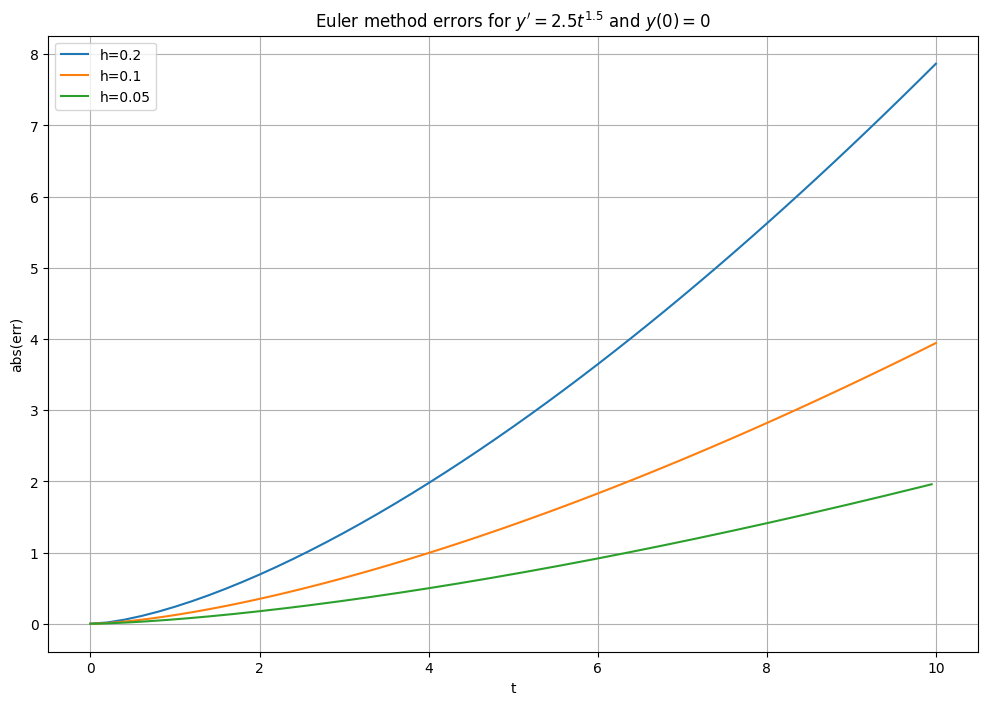
\includegraphics[width=0.95\textwidth]{1}
    \caption{Wykres błędów w zależności od kroku $h$ dla $\alpha_1 = 2.5$}
    \label{fig:mesh}
\end{figure}
Na danym wykresie (Rysunek 1) widać, że dla $\alpha_1 = 2.5$ błąd w kolejnych węzłach, nie dość, że wzrasta, to wzrasta coraz szybciej. Wykres zachowuje te właściwości dla każdego kroku $h$. Jednakże, dla mniejszych kroków $h$, błąd rośnie wolniej, co objawia się "spłaszczeniem"\ tych wykresów.
\begin{figure}[H]
    \centering
    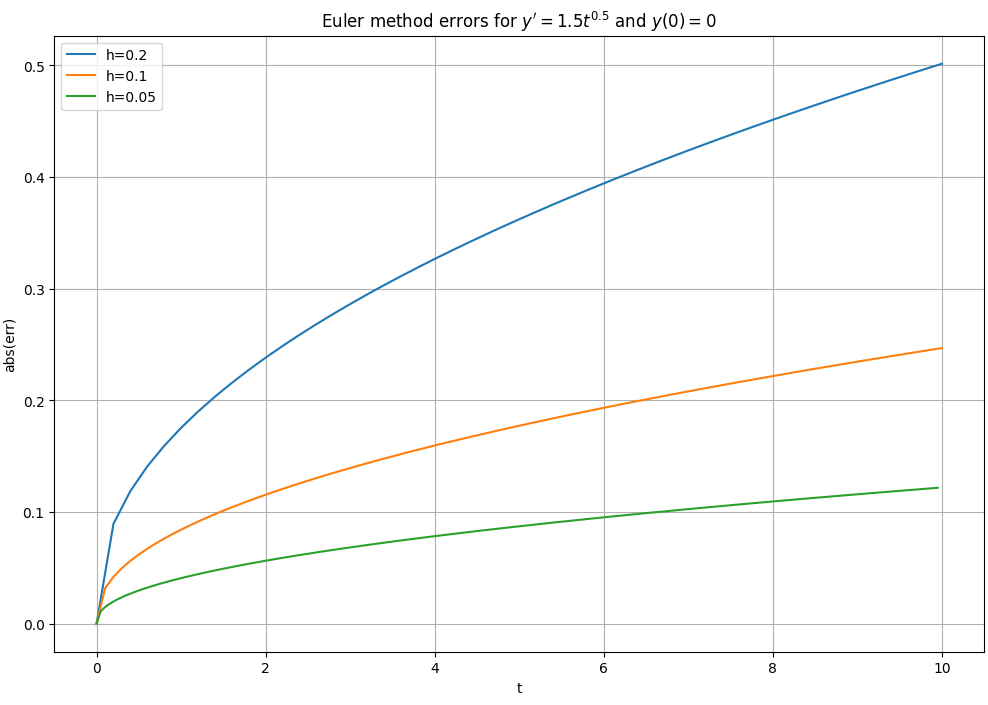
\includegraphics[width=0.95\textwidth]{2}
    \caption{Wykres błędów w zależności od kroku $h$ dla $\alpha_2 = 1.5$}
    \label{fig:mesh}
\end{figure}
Dla $\alpha_2 = 1.5$ widać różnicę od przypadku wcześniejszego. Błąd nadal się zwiększa z każdym węzłem, lecz tym razem rośnie coraz wolniej. Ponownie można tu zauważyć efekt "spłaszczenia"\ wykresów o mniejszych krokach $h$.
\begin{figure}[H]
    \centering
    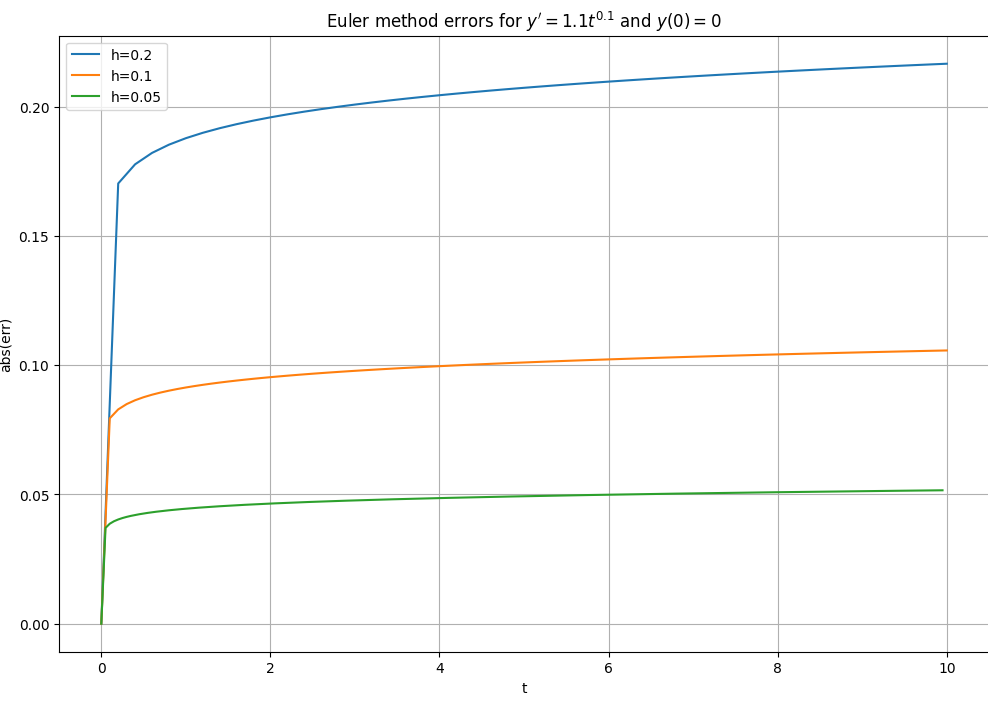
\includegraphics[width=0.95\textwidth]{3}
    \caption{Wykres błędów w zależności od kroku $h$ dla $\alpha_3 = 1.1$}
    \label{fig:mesh}
\end{figure}
W tym przypadku błąd ponownie wzrasta w kolejnych węzłach. Tak jak dla $\alpha_2$ rośnie coraz wolniej z kolejnymi węzłami, natomiast wzrost tutaj jest dużo mniejszy. Gwałtowny wzrost pomiędzy krokiem "zerowym", a krokiem pierwszym (który był również widoczny w poprzednim przypadku) jest tu spowodowany, tym, że dla warunku początkowego mamy dokładną wartość, więc błąd jest równy 0.

\subsubsection{Empiryczny rząd zbieżności metody Eulera}
Do wyznaczenia empirycznie rzędu zbieżności posłuży nam wzór:
$$r = \ln{\frac{\varepsilon_{h_1}}{\varepsilon_{h_2}}} / \ln{\frac{h_1}{h_2}}$$
gdzie $\varepsilon_{h_i}$ to wartości błędu w kolejnych krokach dla kroku $h_i$, $i=1,2$.
\\\\
Poniżej przedstawione zostały wykresy przedstawiające empiryczny rząd zbieżności w kolejnych krokach metody Eulera.
\begin{figure}[H]
    \centering
    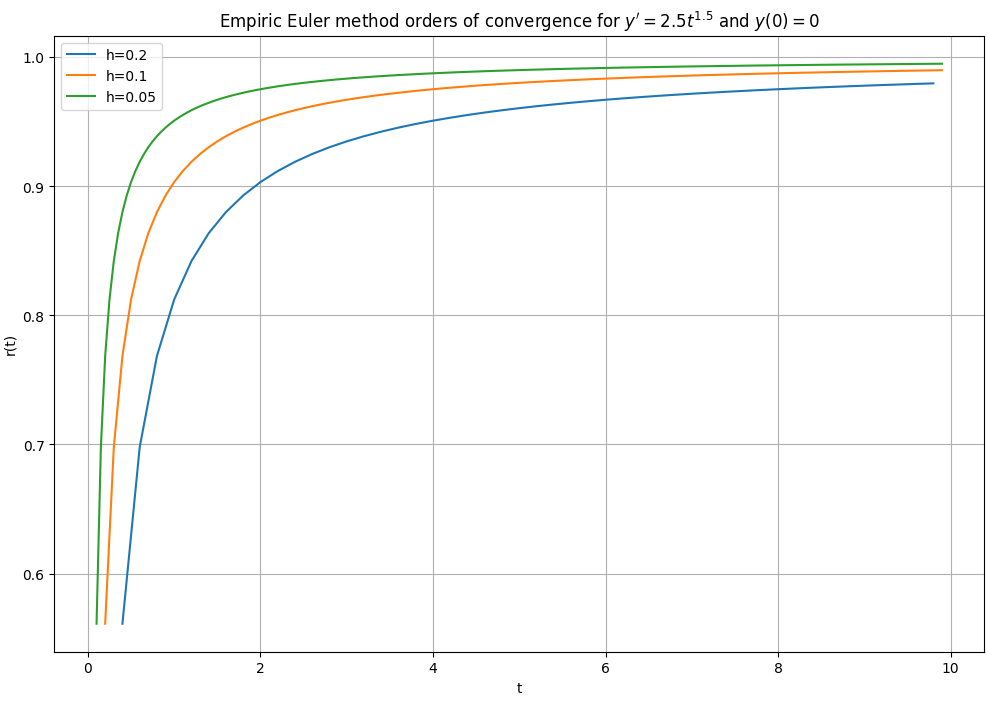
\includegraphics[width=0.95\textwidth]{4}
    \caption{Empiryczny rząd zbieżności w kolejnych krokach dla $\alpha_1 = 2.5$}
    \label{fig:mesh}
\end{figure}
\begin{figure}[H]
    \centering
    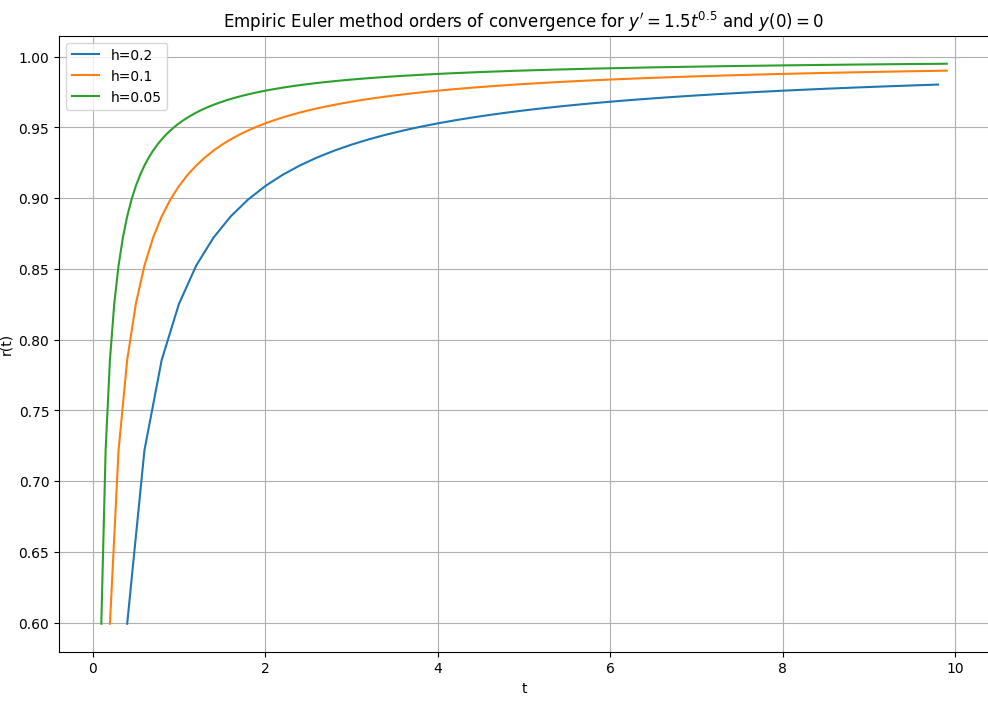
\includegraphics[width=0.95\textwidth]{5}
    \caption{Empiryczny rząd zbieżności w kolejnych krokach dla $\alpha_2 = 1.5$}
    \label{fig:mesh}
\end{figure}
\begin{figure}[H]
    \centering
    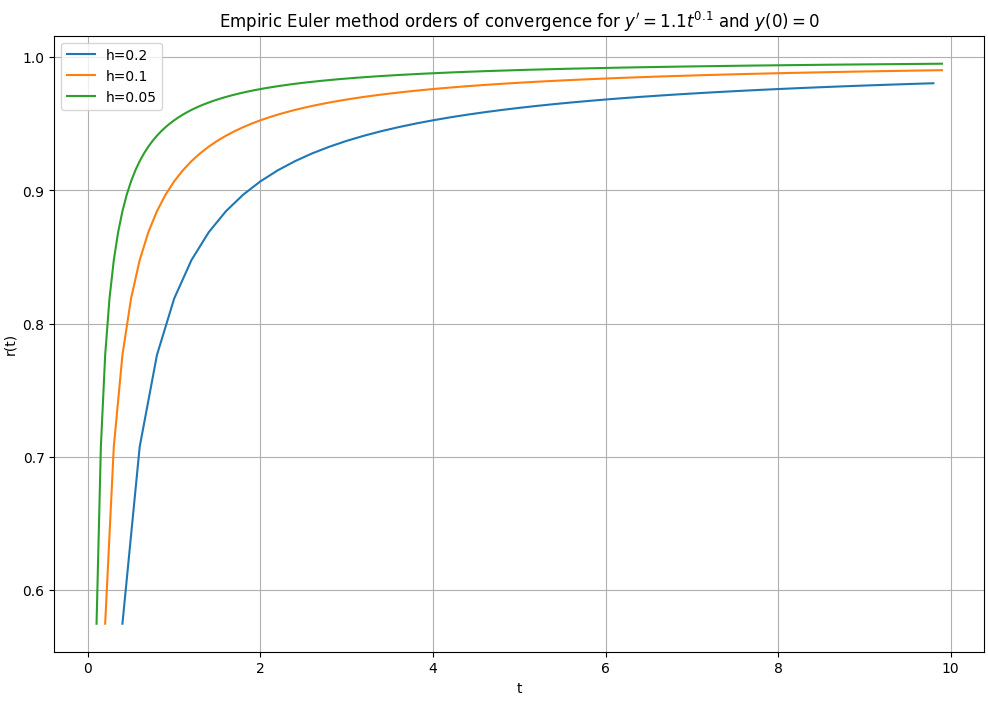
\includegraphics[width=0.95\textwidth]{6}
    \caption{Empiryczny rząd zbieżności w kolejnych krokach dla $\alpha_3 = 1.1$}
    \label{fig:mesh}
\end{figure}
Jak widać z podanych wykresów (Rysunek 4, 5, 6), niezależnie od danego problemu, rząd zbieżności metody Eulera zbiega do 1, co jest zgodne z teorią. Ciekawe jest to, że dla tego problemu, empiryczny rząd zbieżności zaczyna od wartości większej niż teoretyczna i dopiero w następnych krokach się zmniejsza, zbiegając do wartości teoretycznej.

\section{Podsumowanie}
Zadania z tego laboratorium pokazały metody numerycznego rozwiązywania równań różniczkowych.
\\
Zadanie 1. oraz 2. pozwoliły na zaznajomienie się z przekształcaniem problemów do postaci, z której łatwo można dany problem rozwiązać.
\\
Zadanie trzecie pokazało, że należy uważać przy rozwiązywaniu równań różniczkowych na dziedzinę rozwiązania, gdyż dane rozwiązania mogą spełniać zadany problem tylko na jakimś przedziale.
\\
W zadaniu 4., 5. oraz 6. można było poznać jak ważny jest wybór kroku $h$ w rozwiązywaniu równań różniczkowych. Z reguły chcemy wybierać jak największy krok, by zminimalizować obliczenia, jednakże zbyt duży może prowadzić do niedokładności i niestabilności rozwiązania. Zadanie czwarte również pokazało jak duży wpływ na dokładność wyniku ma wybór metody.

\section{Bibliografia}
\begin{itemize}
\item Materiały zamieszczone wraz z zadaniem
\end{itemize}

\end{document}
